\section{Projektmanagement}

In diesem Projekt wurde keine vordefinierte Projektmethodik angewendet. Stattdessen setzten wir auf
\enquote{Best Practices} aus unseren gemeinsam durchgeführten Projekten aus der Vergangenheit, die
auf der agilen Arbeitsweise basieren, die wir aus dem Arbeitsleben gewohnt sind. Diese Konzepte und
Ideen haben wir innerhalb des Rahmens, den die Bachelor Arbeit vorgibt, genutzt und wo nötig entsprechend
ergänzt.

\subsection{Projektplanung}

Der Projektplan orientiert sich am zeitlichen und formellen Rahmen, der die BFH für die Bachelor Arbeit vorgibt und ist in vier
zum Teil überlappende Projektphasen aufgeteilt.
Die Phasen dauern alle in etwa gleich lange, doch der Fokus liegt klar auf der schriftlichen Arbeit, die am meisten
Zeit in Anspruch nimmt.
\begin{enumerate}
    \item Literaturrecherche
    \item Praxisteil
    \item Dokumentationsteil
    \item Präsentationen
\end{enumerate}

Die Abbildung \ref{gantt} bildet unseren Zeitplan in der Form eines Gantt-Diagrammes ab. In der ersten Spalte von links sind die Arbeitspakete
aufgelistet. In der zweiten die geplanten und effektiv verwendeten Zeiten. Die weiteren Spalten repräsentieren dann die zeitliche
Dimension im Projekt, dargestellt durch die nummerierten Arbeitswochen sowie dem Datum vom Montag und dem Sonntag der jeweiligen Woche.
Die fettgeschriebenen, einzeiligen Einträge in der ersten Spalte repräsentieren die Projektphasen. Deren geplante Dauer wird in dunkelblauer Farbe
angezeigt.
Jedes Arbeitspaket nimmt zwei Zeilen ein. Die erste Zeile bildet die Planung ab, die zweite die dokumentierte Realität. Die Zahlen in
der Spalte rechts des Paketnamens enthält die geplante und die effektive Zeit in Personentagen, wobei ein Personentag 8 Stunden repräsentiert.
Die farbigen Balken markieren den Zeitraum, in dem die Arbeitspakete geplant respektive durchgeführt wurden. Blau steht für die Planung und
Orange für den effektiven benötigten Zeitraum.
Die Wochen sind viergeteilt, wobei in jedem Viertel ein Personentag geleistet werden kann. Parallel abgearbeitete Arbeitspakete teilen sich diese
Zeit. Die Hälfte der Woche stellt in unserem Arbeitsplan die Spanne von Montagmorgen bis Donnerstagabend dar. Die zweite Hälfte den Zeitraum bis
zum Ende des Wochenendes.

\newpage
% \pagenumbering{gobble}
\thispagestyle{empty}
\KOMAoptions{paper=landscape,pagesize}
\recalctypearea
    \begin{figure}[H]
        \noindent
	    \begin{center}
            \makebox[\textwidth][l]{\raisebox{0pt}[15cm]{
		    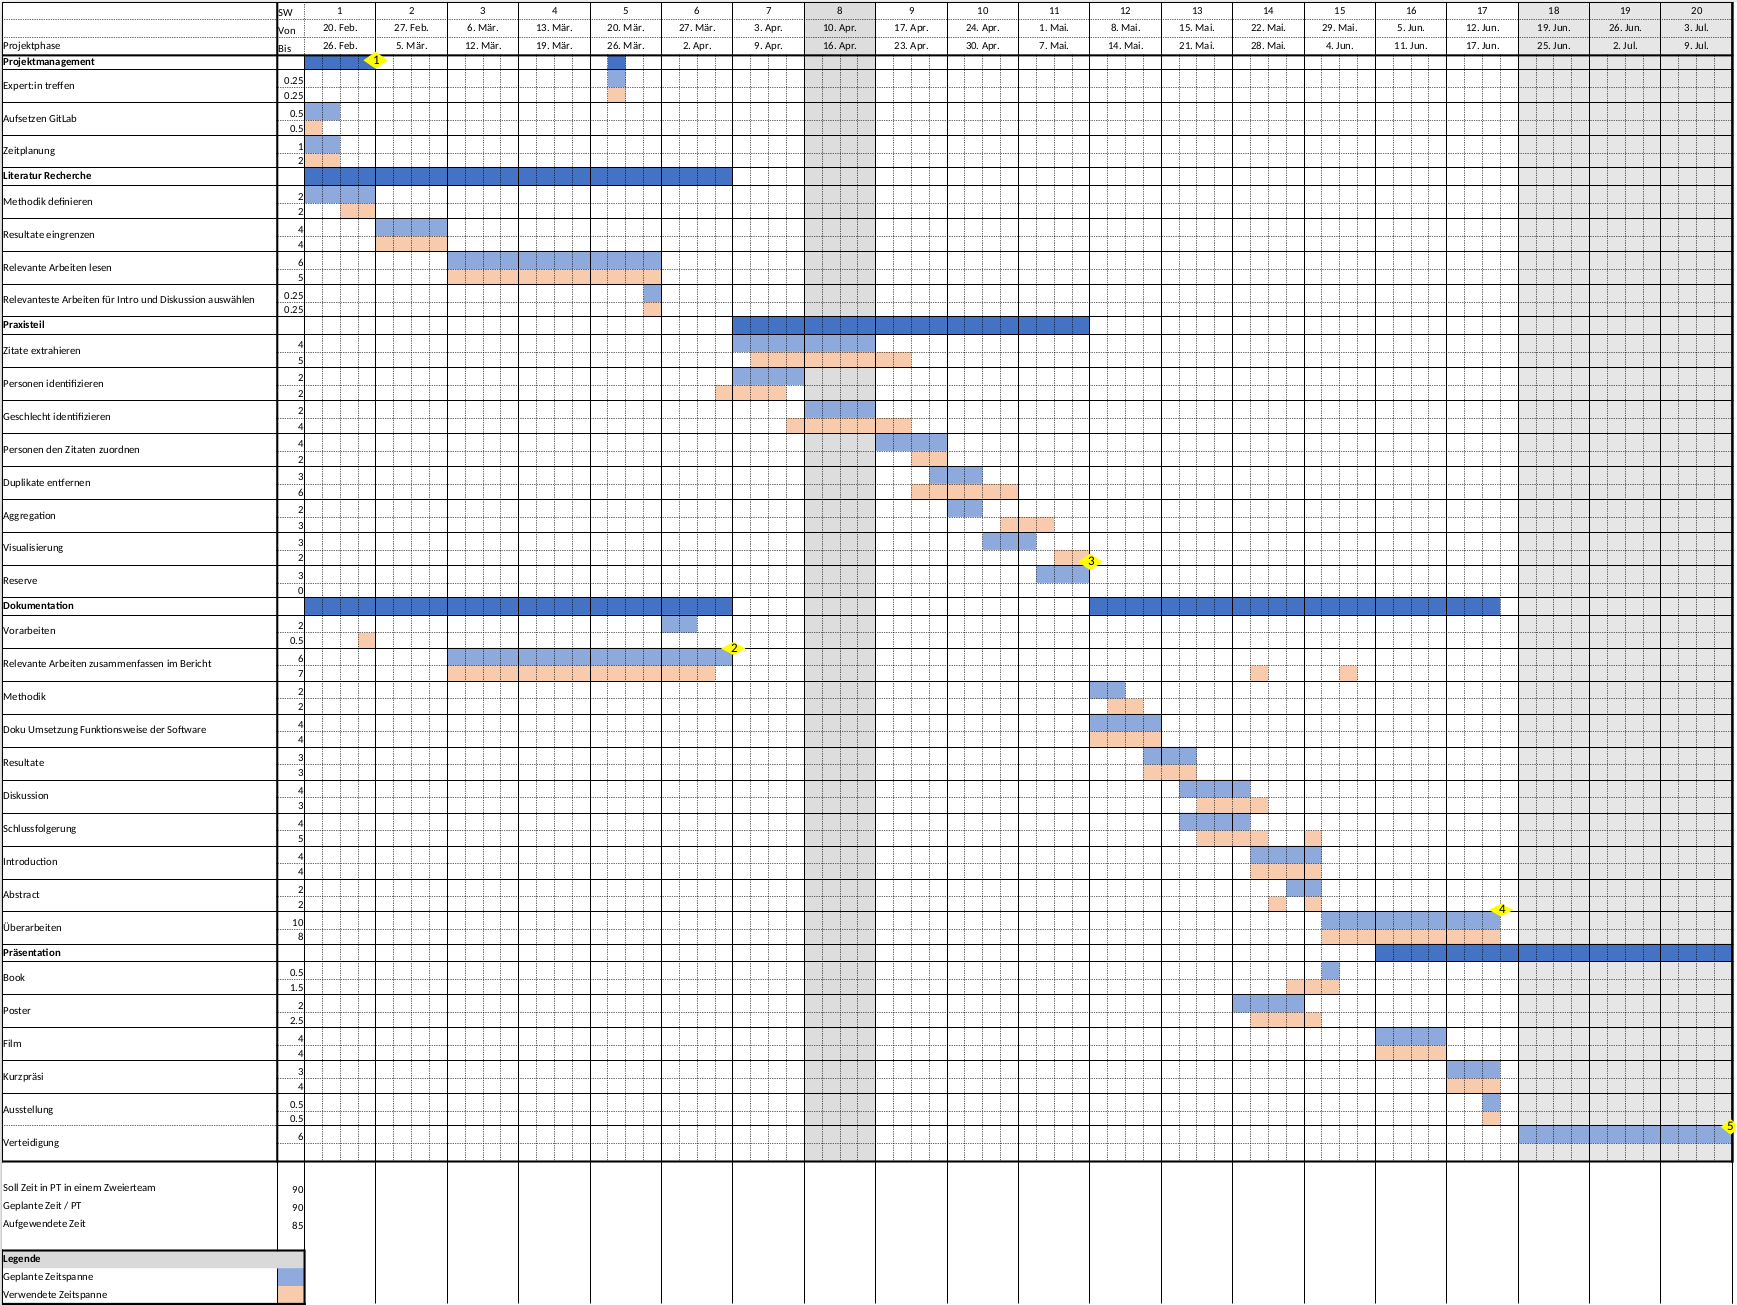
\includegraphics[width=2\linewidth,center]{images/project-planning.png}
            }}
		    \caption{Gantt Diagramm der Projektplanung}
            \label{gantt}
	    \end{center}
    \end{figure}
\newpage
% \pagenumbering{arabic}
\KOMAoptions{paper=portrait,pagesize}
\recalctypearea

\subsection{Arbeitsteilung}

Während den Besprechungen haben wir im Team die Arbeitspakete definiert und im Anschluss auf unserem
Sprint Board auf GitLab eingetragen und beschrieben. Dieses half uns, die offenen Arbeiten und Fragen
nachzuverfolgen und Doppelspurigkeiten zu Identifizieren und zu Eliminieren. Gemäss dem Projektplan haben wir
pro Projektphase ein Sprintboard erstellt, wo wir die aktuell relevanten Arbeiten stets auf einen Blick
sichtbar machen konnten. Dies half uns auch, nicht von offenen Arbeiten aus kommenden Phasen abgelenkt
zu werden. Die nachfolgende Abbildung \ref{sprint-board-screenshot} zeigt einen Screenshot vom Board der Dokumentationsphase.

\begin{figure}[H]
	\begin{center}
        \centering
		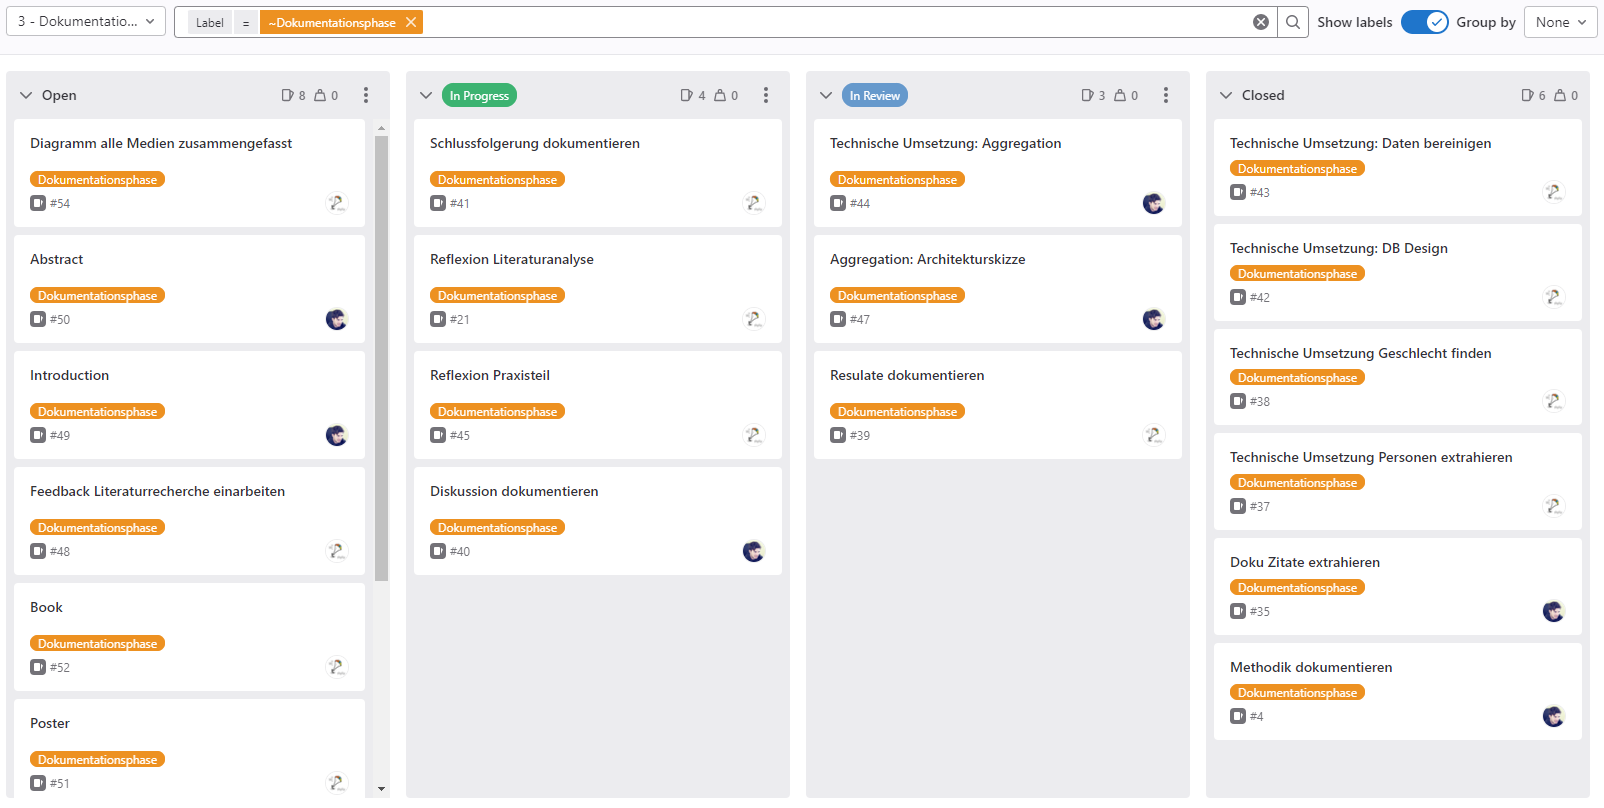
\includegraphics[width=1\linewidth]{./images/kanban_board.PNG}
		\caption{Sprint Board der Dokumentationsphase}
        \label{sprint-board-screenshot}
	\end{center}
\end{figure}

\subsection{Besprechungen}

Für die optimale Zusammenarbeit im Team waren wir stets bemüht, Entscheide gemeinsam zu fällen und
deren Ausführung im Anschluss möglichst unabhängig voneinander abschliessen zu können, um möglichst
effizient Fortschritte erzielen zu können.

Dazu trafen wir uns regelmässig am Montagabend zu einem wöchentlichen Austausch im Team, wo wir den
aktuellen Zwischenstand unserer Arbeiten, allfällige Probleme und weitere Schritte besprachen.
Zudem sahen wir uns zusätzlich stets am Freitag im Unterricht, wo wir uns informell austauschen und
neue Ideen besprechen konnten.

Zusätzlich zu den wöchentlichen Sitzungen im Kernteam trafen wir uns ungefähr jede zweite Woche mit
unserer Betreuerin, Prof. Dr. Mascha Kurpicz-Briki, um ihr den aktuellen Stand der Arbeiten und den
Fortschritt gemessen am Projektplan präsentieren zu können. In diesen Meetings konnten wir zusätzlich
inhaltliche und Formelle Fragen klären und durch Feedback von der grossen Erfahrung unserer Betreuerin
profitieren.
